本章介绍一种从单张RGB-D图像中进行6自由度物体位姿估计的实例级物体位姿估计方法。当前实例级物体位姿估计中的领先方法\cite{Sundermeyer2023BOPC2}依赖基于渲染的精调流程,在实时性上有一定的瓶颈。基于渲染的精调流程需要渲染器渲染出当前估计所对应的图像,渲染过程需要耗费较多的资源。为了规避渲染耗时的局限性,我们提出了基于层次化表面编码和对应关系剪枝的HiPose架构,该方法通过层次化的二进制表面编码以粗到精的方式建立观测点到模型表面区域的对应关系。与之前的稠密对应方法不同,我们不直接估计观测点对应的模型对应点,而是通过采用点到表面匹配来估计对应表面,并迭代性地收缩表面,直到其转变为对应点,同时逐渐去除离群点。在公共基准数据集 LM-O、YCB-V 和 T-LESS 上进行的大量实验显示,我们的方法在不依赖精调流程的方案中表现最优,甚至能与那些相对耗时的基于渲染的方法相抗衡。尤为重要的是,我们的方法计算效率极高,这使其能够在对精度要求苛刻的实时关键应用场景中发挥作用。代码链接见 \url{https://github.com/lyltc1/HiPose}。

\section{引言}
在缺乏纹理和严重遮挡的场景中,六自由度物体位姿估计仍具有挑战。近期的一些仅基于RGB的研究\cite{su2022zebrapose}在处理遮挡方面表现良好,但因单目图像存在深度不确定性而造成了精度下降。而一些基于RGB-D的方法\cite{wang2019densefusion,he2020pvn3d,he2021ffb6d,zhou2023deep}提出了新的特征融合网络,以更好地利用RGB和深度信息,但在公共基准如BOP挑战赛\cite{Sundermeyer2023BOPC2}上的表现仍落后。相较之下,目前大多数最先进的方法通常先利用RGB图像估计位姿,然后利用深度信息进行基于迭代优化的位姿精调流程\cite{Rusinkiewicz2001EfficientVO,lipson2022coupled}。与之不同的是,我们提出的HiPose直接利用RGB-D图像进行位姿估计能够提供更精确、更可靠的物体位姿估计。

该方法通过深度融合几何与色彩信息实现精准估计,且无需依赖耗时的后处理优化步骤。得益于RGB-D传感器提供的多模态数据(包括观测点到相机的距离等几何信息),我们的方法能够构建更鲁棒的视觉表征。受ZebraPose\cite{su2022zebrapose}框架的启发,我们设计了HiPose新型网络架构,该架构通过预测深度图像与物体模型之间的密集对应关系实现位姿估计。与ZebraPose采用的编码使用策略不同,我们提出一种基于迭代离群点消除的渐进式优化机制,通过由粗到精的多阶段处理流程逐步剔除异常对应点,如\autoref{fig:HiPose方法概览}所示。这种改进的编码处理方式不仅充分利用了编码的层次化特征,还显著提升了对应关系的精度和鲁棒性,能够实现实时高精度位姿估计。

\begin{figure}[ht]
    \centering
    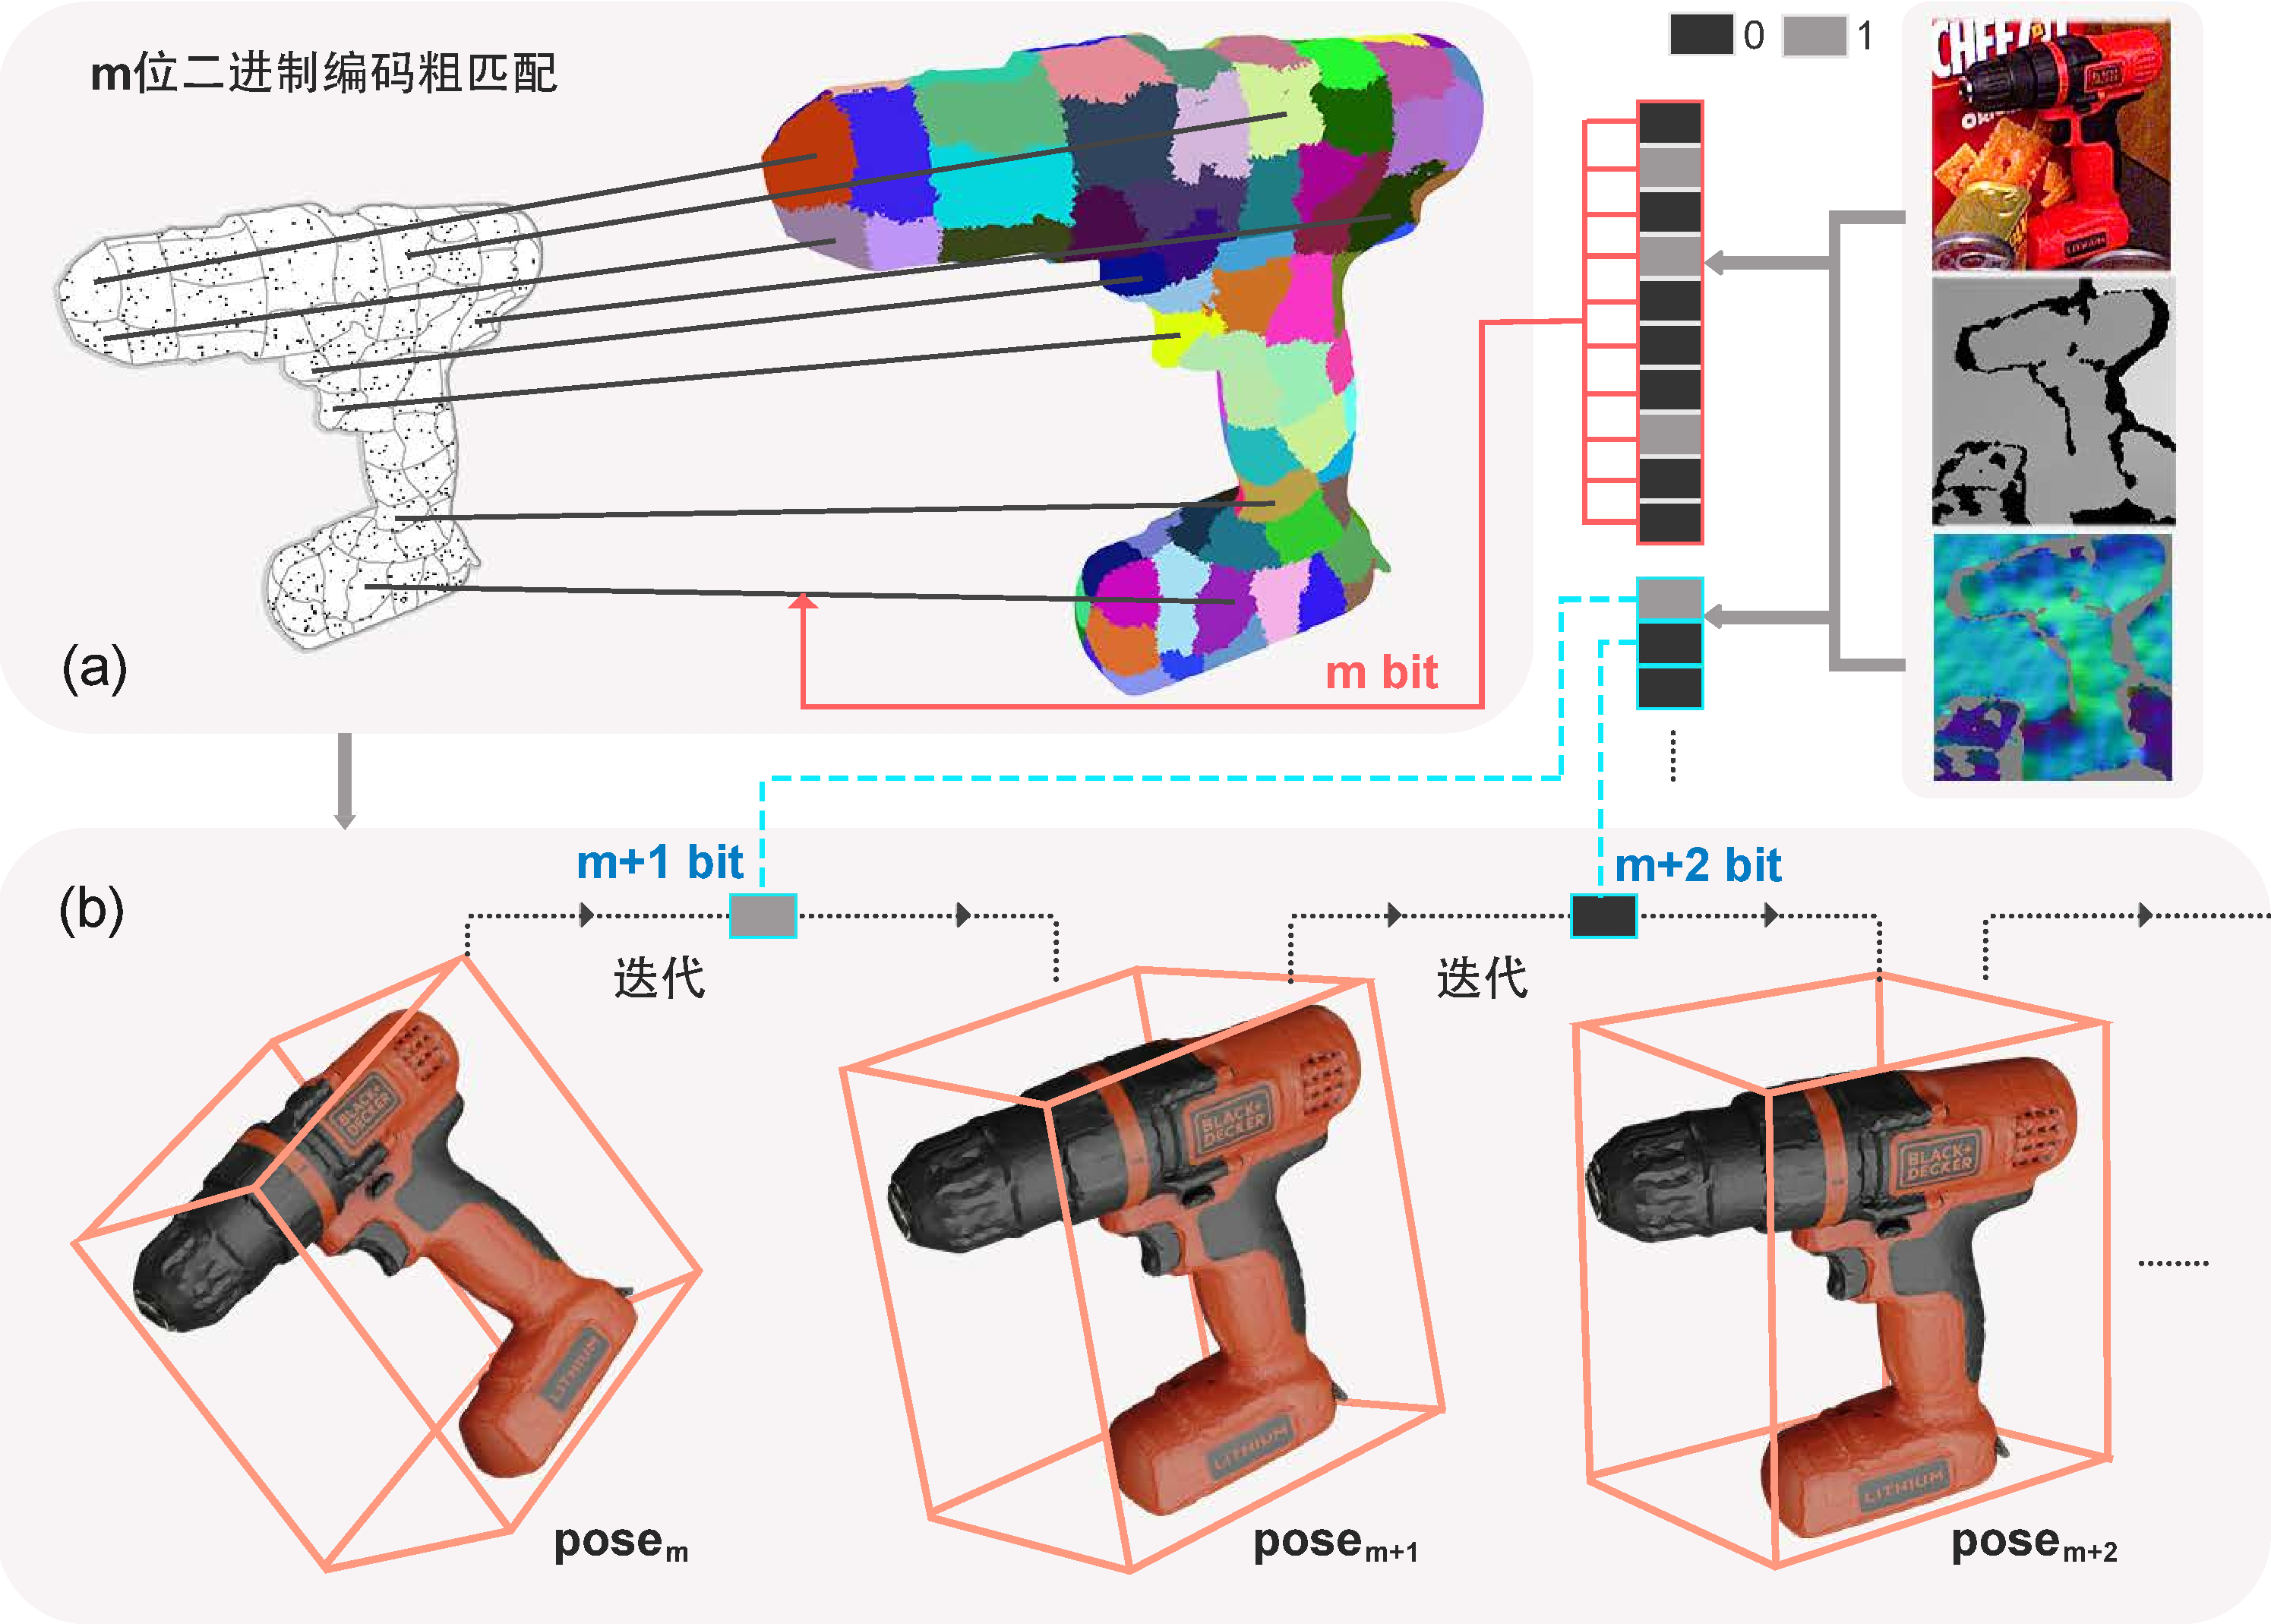
\includegraphics[width=0.75\linewidth]{hipose/teaser.pdf}
    \caption{HiPose的粗匹配和细匹配}
    \label{fig:HiPose方法概览}
\end{figure}

我们提出了一种新颖且更为稳定的层次化对应剪枝方法,而不是在常见的RANSAC框架下使用预测的对应关系来解决位姿问题,如与Kabsch算法\cite{umeyama1991least}常结合的方法那样。具体而言,层次化二进制编码输出中的粗略预测更不容易出错,提供了一个稳健的初始位姿。这一粗略位姿有助于基于点到表面距离识别和去除离群匹配。随后,我们在每次迭代中应用更精细的预测,逐步完善我们的位姿预测,并在更细的层面上去除离群点,以提高精度。

总体而言,我们的贡献可以总结如下:
\begin{itemize}
\item 我们提出了一种充分利用RGB-D数据的物体位姿估计方法,专注于通过层次化二进制表面编码进行3D-3D对应匹配。
\item 我们引入了一种基于层次化对应剪枝的RANSAC-free位姿估计方法,通过粗到精的子表面去除离群点。
\item 在LM-O、YCB-V和T-LESS数据集上的大量实验表明我们方法的有效性。我们在没有任何额外精细化的情况下实现了最先进的结果,使我们的方案明显快于其他方法,适合实时应用。
\end{itemize}
